\documentclass{ximera}

\newcommand{\RR}{\mathbb R}
\renewcommand{\d}{\,d}
\newcommand{\dd}[2][]{\frac{d #1}{d #2}}
\renewcommand{\l}{\ell}
\newcommand{\ddx}{\frac{d}{dx}}
\newcommand{\dfn}{\textbf}
\newcommand{\eval}[1]{\bigg[ #1 \bigg]}


\title[Dig-In:]{The Work-Energy Theorem}

\begin{document}
\begin{abstract}
  Substitution is given a physical meaning. 
\end{abstract}
\maketitle

In physics, we take measurable quantities from the real world, and
attempt to find meaningful relationships between them. A basic example
of this would be the physical ideal of \dfn{force}. Force applied to an
object changes the motion of an object. Here's the deal though, at a
basic level
\[
\mathrm{force} = \mathrm{mass} \cdot \mathrm{acceleration}.
\]
and while we can put a physical interpretation to this arithmetical
definition, at the end of the day force is simply ``mass times
acceleration.'' The SI unit of force is a \dfn{newton}, which is defined to be
\[
1\unit{N} = 1\unit{kg}\cdot \unit{m}/\unit{s}^2. 
\]
\begin{question}
  To get a feel for what a newton is, consider this, if an apple has a
  mass of $0.1\unit{kg}$, what force would an apple exert on your hand
  due to the acceleration due to gravity?
  \begin{prompt}
  \[
  F = (0.1) \cdot (-9.8) = \answer{-0.98}\unit{N},
  \]
  \end{prompt}
\begin{feedback}
  Hence the ``weight'' of an apple is approximately $1\unit{N}$.
\end{feedback}
\end{question}


In a similar way, the idea of \dfn{kinetic energy}, is ``energy''
objects have from motion. It is defined by the formula
\[
E_k = \frac{m \cdot v^2}{2}.
\]
The SI unit of energy is a \dfn{joule}, which is defined to be
\[
1\unit{J} = 1\unit{kg}\cdot \unit{m}^2/\unit{s}^2 = 1\unit{N}\cdot\unit{m}. 
\]
To put this in perspective, $1$ joule is approximately the energy
released by an apple that has fallen $1$ meter to the ground.
\begin{question}
  Suppose a car 5mph and 0, vs 75 70 1000 kg.
\end{question}



Finally \dfn{work} is defined to be accumulated force over a
distance. We can write this in the language of calculus as,
\[
W = \int_{s_0}^{s_1} F(s) \d s.
\]
The SI unit of work is also a \dfn{joule}. To help understand this,
$1$ joule is approximately how much work is done when you raise an
apple one meter.
\begin{question}
  Which of the following are examples where work is being done?
  \begin{selectAll}
    \choice{studying calculus}
    \choice[correct]{a car applying breaks to come to a stop over a distance of $100\unit{ft}$}
    \choice[correct]{a young mathematician climbing a mountain}
    \choice{a young mathematician standing still, holding a $1000$ page calculus book for $10$ minutes}
    \choice{a young mathematician walking around with a $1000$ page calculus book}
    \choice[correct]{a young mathematician picking up a $1000$ page calculus book}
  \end{selectAll}
  \begin{feedback}
    While studying calculus may ``feel'' like work, it is not
    (typically) an example of an accumulated force over a distance,
    and hence no work is done.

    On the other hand, a car applying breaks is a change in motion, and
    hence a force is applied. Since this force is applied over a
    distance, work is done.

    Climbing a mountain is also an example of work, as one is applying
    force to overcome the acceleration due to gravity, over the
    distance that one is climbing.

    No work is done when holding a calculus book, as there is no
    accumulated force over a distance.

    It is also the case that no work is done when one walks around
    with a calculus book, this is because the ``force'' is in a
    direction perpendicular to the motion.

    Finally, when one picks up a calculus book, you are moving the
    book against the force due to the acceleration due to
    gravity. Hence work is done.
  \end{feedback}
\end{question}



Now we have a question:
\begin{quote}
 \textbf{Why do work and kinetic energy have the same units?}
\end{quote}

One way to answer this is via the \textit{Work-Energy Theorem}.

\begin{theorem}[Work-Energy Theorem]
  Suppose that an object of mass $m$ is moving along a straight
  line. If $s_0$ and $s_1$ are the the starting and ending positions,
  $v_0$ and $v_1$ are the the starting and ending velocities, and
  $F(s)$ is the force acting on the object for any given position,
  then
  \[
  W = \int_{s_0}^{s_1} F(s) \d s = \frac{m\cdot v_1^2}{2} - \frac{m\cdot v_0^2}{2}.
  \]
  \begin{explanation}
    First we need to get all of our symbolism out in the open. Let:
    \begin{itemize}
    \item $s(t)$ represent position with respect to time,
    \item $v(t)$ represent velocity with respect to time,
    \item $a(s)$ represent acceleration with respect to position,
    \item $t_0$ represent the starting time,
    \item $t_1$ represent the ending time,
    \end{itemize}
    then we also have that
    \begin{itemize}
    \item $s(t_0)$ represents the starting position, $s_0$,
    \item $s(t_1)$ represents the ending position, $s_1$,
    \item $v(t_0)$ represents the starting velocity, $v_0$,
    \item $v(t_1)$ represents the ending velocity, $v_1$.
    \end{itemize}
    Now write with me,
    \[
    W = \int_{s_0}^{s_1} F(s) \d s = \int_{s(t_0)}^{s(t_1)} F(s) \d s
    \]
    we will use the substitution formula,
    \begin{image}
    \begin{tikzpicture}[scale=1,every node/.style={transform shape}]
      \draw [->, line width=10, penColor!10!background] (1,0)--(-0.5,0);
    \node at (0,0) {
      $\int_a^b f'(g(x)) g'(x) \d x =\int_{g(a)}^{g(b)} f'(g) \d g$
    };
    \end{tikzpicture}
  \end{image} 
    transforming from right to left, to see that
    \[
    \int_{s(t_0)}^{s(t_1)} F(s) \d s = \int_{t_0}^{t_1} F(s(t)) s'(t) \d t.
    \]
    Since $s'(t) = v(t)$, we may write
    \[
    \int_{t_0}^{t_1} F(s(t)) s'(t) \d t = \int_{t_0}^{t_1} F(s(t)) v(t) \d t
    \]
    and now remember that $F=m\cdot a$, so
    \[
    \int_{t_0}^{t_1} F(s(t)) v(t) \d t = \int_{t_0}^{t_1} m\cdot a(s(t)) v(t) \d t.
    \]
    However, $a(s(t)) = v'(t)$, so rearranging we have,
    \[
    \int_{t_0}^{t_1} m\cdot a(s(t)) v(t) \d t = m\cdot \int_{t_0}^{t_1} v(t) v'(t)\d t.
    \]
    Now we apply the substitution formula again, this time we will transform left to right
    \begin{image}
    \begin{tikzpicture}[scale=1,every node/.style={transform shape}]
      \draw [->, line width=10, penColor!10!background] (-.5,0)--(1,0);
      \node at (0,0) {
        $\int_a^b f'(g(x)) g'(x) \d x =\int_{g(a)}^{g(b)} f'(g) \d g$
      };
    \end{tikzpicture}
    \end{image}
    and so we see
    \[
    m\cdot \int_{t_0}^{t_1} v(t) v'(t)\d t = m\cdot \int_{v(t_0)}^{v(t_1)} v \d v.
    \]
    At last, setting $v(t_0) = v_0$ and $v(t_1) = v_1$, we can evaluate
    this integral,
    \begin{align*}
      m \cdot \int_{v_0}^{v_1} v \d v &= m \cdot \eval{\frac{v^2}{2}}_{v_0}^{v_1}\\
      &=\frac{m\cdot v_1^2}{2} - \frac{m\cdot v_0^2}{2}.
    \end{align*}
  \end{explanation}
\end{theorem}

The Work-Energy theorem says that:
\begin{center}
  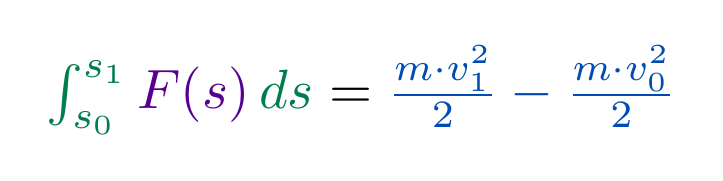
\begin{tikzpicture}[scale=2,every node/.style={transform shape}]
    \node at (0,0) {
      $\color{green!70!black!70!blue}\int_{s_0}^{s_1}\color{purple!50!blue!90!black}F(s) \color{green!70!black!70!blue}\d s\color{black} = \color{blue!70!green}\frac{m\cdot v_1^2}{2} - \frac{m\cdot v_0^2}{2}$
      };
  \end{tikzpicture}
\end{center}
This could be interperted as:
\begin{quote}\large\textbf{The \textcolor{green!70!black!70!blue}{accumulated} \textcolor{purple!50!blue!90!black}{force} \textcolor{green!70!black!70!blue}{over distance} is the \textcolor{blue!70!green}{change in kinetic energy}.}
\end{quote}
Moreover, this answers our initial question of why work and kinetic
energy have the same units, essentially, energy powers work.


\end{document}
      
